	\chapter{METHODOLOGY}
	\label{chap:methodology}
	
	\section{Vehicle Classification}
	
	 Electric vehicles have been classified primarily into four major categories as shown in Figure~\ref{fig:classification} 
	 	
			\begin{figure}[h]
				\centering
				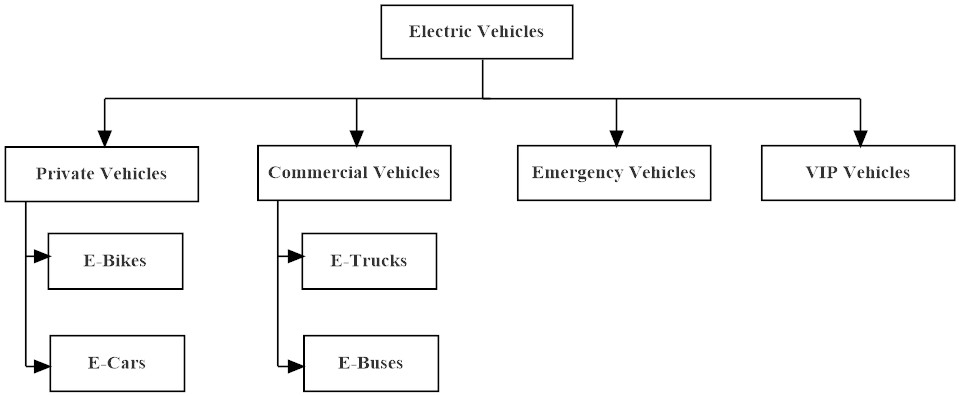
\includegraphics[width=0.7\linewidth]{./Figures/classification}
				\caption{Vehicle Classification}
				\label{fig:classification}
			\end{figure}
		
	The above classification is made by comparing the battery capacity of the vehicles from the data taken with the battery capacity of the similar kind of vehicles in the market.

	\par {Private vehicles are further classified into E-bikes and E-cars with average battery capacity of 400 $Wh$ to 500 $Wh$ and 40 $kWh$ to 100 kWh respectively. Commercial vehicles are classified into E-Truck and E-Bus with an average battery capacity of 100 $kWh$ and 60 to 548 kWh respectively. Emergency vehicles have a battery capacity of around 105 $kWh$ and VIP vehicles have around 90 $kWh$ to 200 $kWh$.
	}
	
	\section{Travel Pattern Establishment}
	
	Travel pattern for three main vehicle subcategories of the above mentioned vehicle categories namely E-car, E-Truck and E-Bus are now taken and travel patterns of the same have been established by using the Battery capacity, Time taken to full charge, Time period of the vehicle when it is connected to the grid , charging rate and discharging rate \cite{evdata}.
	
	Bus: ID – 16034
	This id is chosen as the battery capacity of the bus is considered to be the best in market. The
	battery capacity range of bus is 199.95 KWH. The time taken for 100\% charging of battery
	happens to be 5 hours 20 minutes. It can run for 24 hours after full charging. The charging of
	bus would take place every alternative day as the bus takes 24 hours to complete its trip. The
	bus would have energy of 12.5 KWH on completion of 20 minutes of charging when plugged
	at 0\% Soc. It would have a time period of 5 hours 40 minutes to keep the vehicle idle or to
	discharge.
	
	Car: ID – 13646
	Car ID 13646 is chosen as it is the best in market for all the EV cars in recent times. The
	battery capacity range of car is 54 KWH. The time taken for full charge when plugged at 0\%
	SoC is 1 hour 40 minutes. It can run for 6 hours 30 minutes after full charge. As the vehicle is
	a car its trip for a day can be 2 times and so the above pattern can be repeated for the second
	part of the day. Charge of the vehicle after 20 minutes of charging when plugged at 0\% SoC
	is 10.8 KWH. After the completion of full charge it will have 3 hours 40 minutes for idle/
	discharge period.
	
	Truck: ID – 4428
	Truck ID 4428 is considered as it is successful in market when compared with other trucks.
	The battery capacity range of bus is 99.2 KWH. It requires complete 4 hours to have 100\%
	battery charge or 100\% Soc. It takes 14 hours to fully utilize 99.2 KWH after full charge of
	the battery. As it takes 14 hours to complete its trip it is restricted for one day travel. The
	charge at the end of 20 minutes is 8.267 KWH. After the charging for 4 full hours it will have
	6 hours for the vehicle to discharge or keep the vehicle idle.
	
	\section{Charging/Discharging pattern Establishment}
	
	Generally for the travel pattern to be established, the time scale will be taken for 24 hours
	counting every hour. Here the time scale is considered to be 72 blocks as 1 hour is split into
	three 20 minute block for 24 hours because the classified vehicles have different battery
	capacity range. This split up is done to find the best efficient charging/discharging pattern in
	order to reduce the cost that is paid to the grid for the beneficial of consumers.
	
	\section{Flowchart}
	
	\begin{figure}
		\centering
		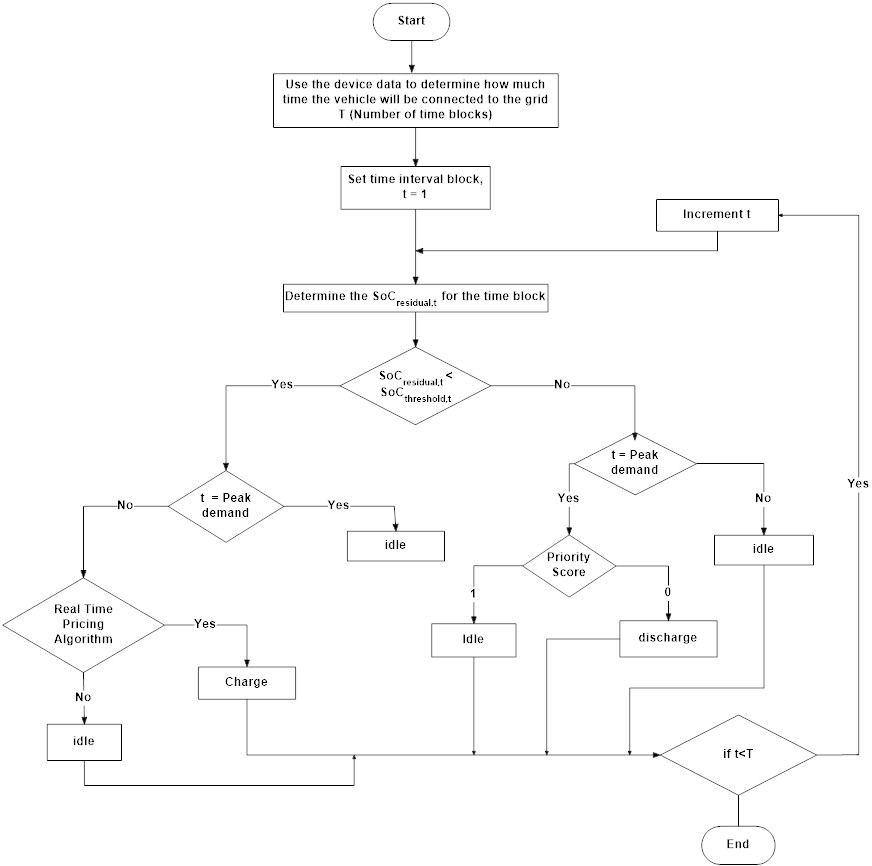
\includegraphics[width=0.9\linewidth]{Figures/Ev_flowchart}
		\caption{}
		\label{fig:evflowchart}
	\end{figure}


	\section{Real Time Price}
	
		\begin{figure}[!h]
			\centering
			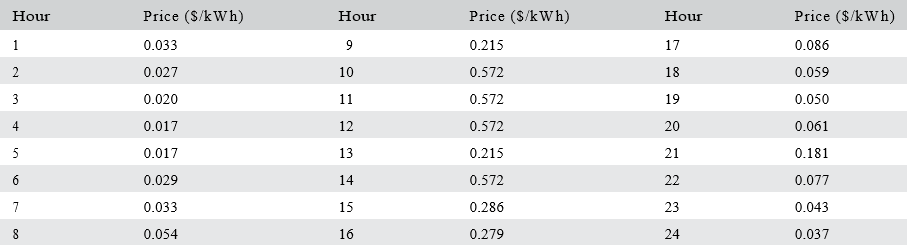
\includegraphics[width=0.7\linewidth]{Figures/rtp}
			\caption{}
			\label{fig:rtp}
		\end{figure}
	
	